\chapter{Experimental Evaluation of Rényi-based Knowledge Distillation}

This chapter is dedicated to applying the modified knowledge distillation process, in which Rényi divergence is used in place of the traditional Kullback–Leibler (KL) divergence. The experimental evaluation is conducted using the ResNet architecture on the CIFAR-100 dataset.

In the first experiment, we compare the performance of standard knowledge distillation with that of the Rényi-based approach. The second experiment extends this comparison by evaluating the results of two newly formulated Rényi-based knowledge distillation setups against those from the previous experiment.

\section{Dataset}

The dataset used for our experiments is CIFAR-100, which was introduced in \cite{Krizhevsky2009} as a subset of a larger dataset created by \cite{TorralbaFergusFreeman2008}. It consists of 60,000 labeled color images across 100 classes, with 600 images per class. There are 50,000 images in the training set and 10,000 images in the test set. All images are downscaled to $32 \times 32$ pixels. The 100 classes in the dataset are grouped into 20 so-called superclasses.

As an example we select two superclasses called \textit{large omnivores and herbivores} and \textit{household furniture}. The first contains classes \textit{camel}, \textit{cattle}, \textit{elephant}, \textit{chimpanzee} and \textit{kangaroo}, while the second one contains classes \textit{bed}, \textit{couch}, \textit{chair}, \textit{table} and \textit{wardrobe}. Clearly, the classes within the same superclass are much more similar than those across superclasses, often sharing the same textures, shapes, or color patterns as can be seen in Figure~\ref{fig:cifar100}.

\begin{figure}[h!]
	\centering
	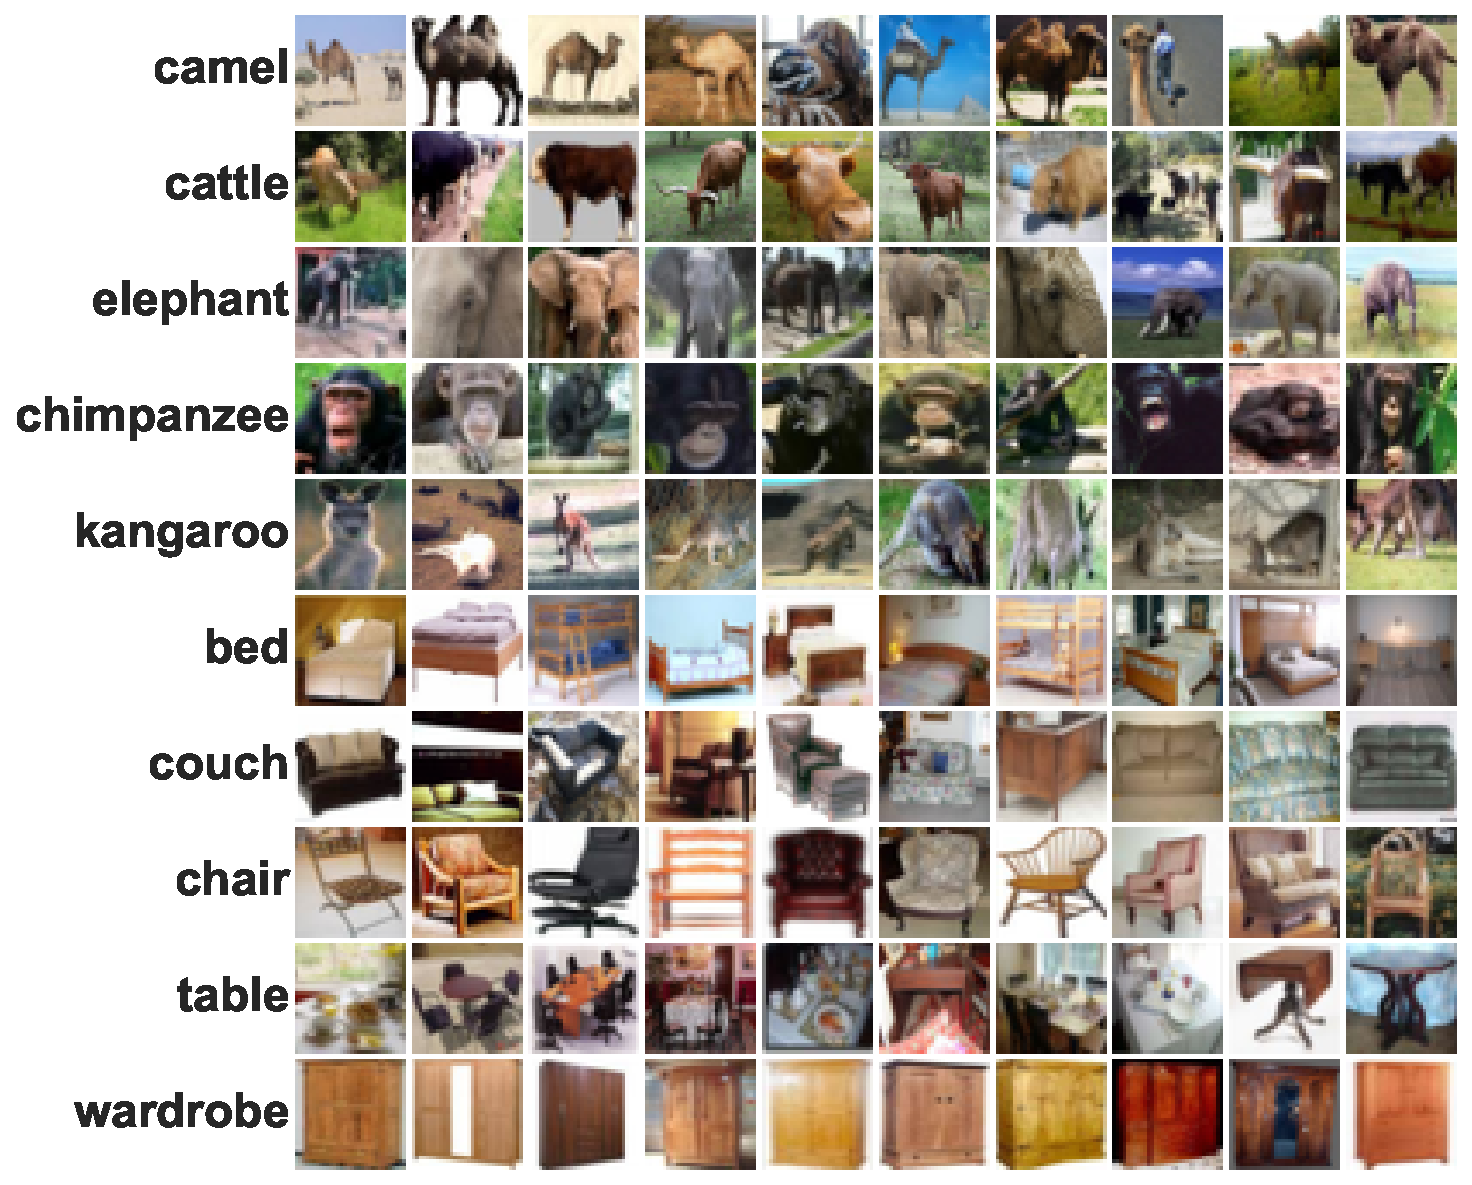
\includegraphics[width=0.57\textwidth]{../img/cifar100_grid.pdf}
	\caption{Visualization of 10 randomly selected images from each of the 5 classes within the superclasses \textit{large omnivores and herbivores} (top) and \textit{household furniture} (bottom) from the CIFAR-100 dataset.}
	\label{fig:cifar100}
\end{figure}

\section{Experiment 1}

In this first experiment, we evaluate the performance of Rényi-based knowledge distillation, which introduces a hyperparameter $\alpha \in [0, \infty]$. When $\alpha = 1$, the loss function is equivalent to that of standard knowledge distillation, providing a natural baseline for comparison.

For the experimental setup, we chose ResNet152 as the architecture for the teacher model and ResNet18 for the student model. We thus chose the teacher model to be much larger ($11.3 \times 10^9$ parameters) compared to the student model ($1.8 \times 10^9$ parameters) to exaggerate the performance difference between the models, thereby increasing the potential for improvement during knowledge distillation and allowing us to more reliably evaluate the impact of the various modifications introduced to the student model testing.

Training was performed using the Python programming language and the Timm library (\cite{Wightman2019}), which provides various advanced methods for optimization, regularization, and data augmentation, along with many pre-built models, including various ResNet architectures. However, it does not include support for knowledge distillation and Rényi loss. Thus, we needed to modify parts of the code to support both standard and Rényi-based knowledge distillation.

Given the large number of hyperparameters to tune in the Timm library, we decided to adopt a configuration strategy inspired by \cite{AbbasLee2021}, which aimed to optimize the performance of ResNet models on the CIFAR-100 dataset. The hyperparameters used are summarized in Table~\ref{tab:hyperparams} below. A notable modification we made was increasing the batch size and learning rate by a factor of four, which, as shown in \cite{Goyal2017}, does not substantially affect overall performance. Our motivation for this change was to speed up the training process. Additionally, we did not apply dropout to the fully connected layer and extended the number of epochs by 20, both of which are minor changes that had no significant impact on performance. The motivation behind these changes was to stabilize performance fluctuations between successive epochs at the end of the training.

\begin{table}[h]
	\centering
	\begin{tabular}{lc}
		\toprule
		\textbf{Hyperparameter}     & \textbf{Value} \\ \midrule
		Optimizer                    & SGD            \\
		Learning rate\tablefootnote{Learning rate decay was applied during training as a standard machine learning procedure.} & 0.08 \\
		Momentum                     & 0.9            \\
		Weight decay                 & 0.0005       \\
		Epochs                       & 220            \\
		Batch size                   & 512            \\
		Activation function          & ReLU           \\
		\bottomrule
	\end{tabular}
	\caption{Training hyperparameters used for the experiment inspired by \cite{AbbasLee2021}.}
	\label{tab:hyperparams}
\end{table}

We also introduce data augmentation, which refers to modifications applied to the dataset to improve the model’s generalization ability, such as rescaling, cropping, and flipping images, as suggested by \cite{Wightman2021}.

First, using the training setup described above, we train both the ResNet152 and ResNet18 models on the train set without applying knowledge distillation, that is, using vanilla training, as described in the first chapter. The first model is the teacher model for knowledge distillation, while the second model, referred to as the vanilla model, shares the same architecture as the student model but is trained independently, without knowledge distillation. This model serves as our benchmark against which the results of knowledge distillation are compared.

In Figure~\ref{fig:teacher_vanilla_model}, we observe the performance of the models, measured by the test accuracy on the CIFAR-100 dataset. As expected, the teacher model performs better, achieving a final accuracy of 68.06\%, compared to the vanilla model, which ended training with an accuracy of 62.61\%. Since the test set contains 10,000 images, the difference between the two models corresponds to 545 images being correctly/incorrectly classified. Looking closely, we observe that the two models performed similarly during the first 50 epochs. Afterward, the teacher model began improving at a faster rate than the student.

\begin{figure}[h!]
	\centering
	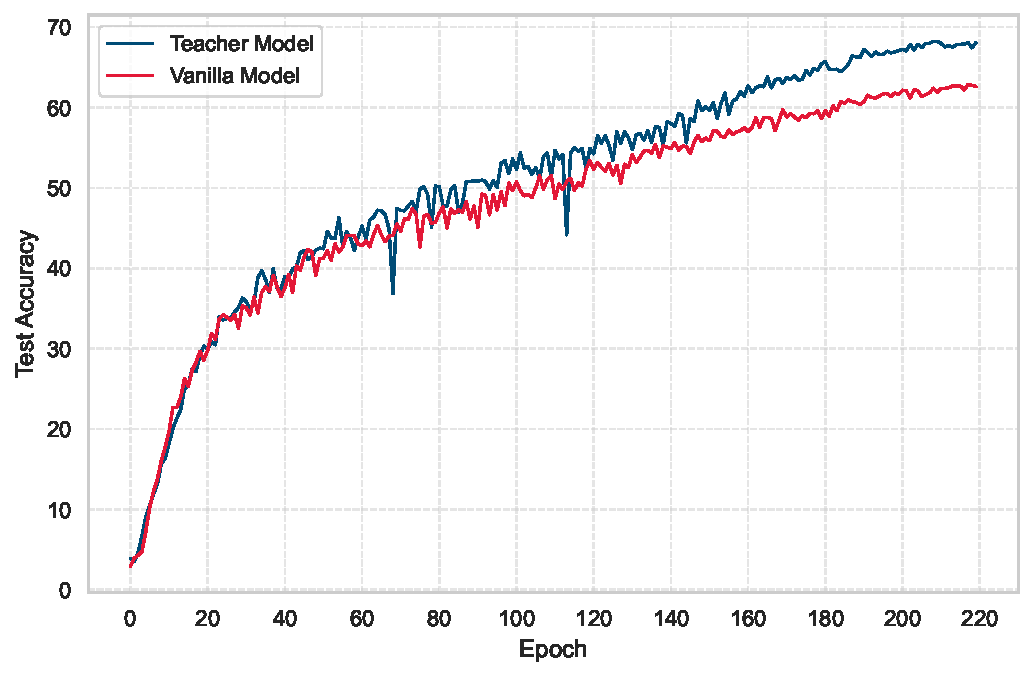
\includegraphics[width=0.7\textwidth]{../img/teacher_vanilla_model.pdf}
	\caption{Test accuracy over 220 epochs for the teacher and vanilla models.}
	\label{fig:teacher_vanilla_model}
\end{figure}

Now, we turn our attention to knowledge distillation, which requires additional three hyperparameters, as shown in Equations~(\ref{Rényi Knowledge Distillation}) and (\ref{Rényi loss}): $\alpha$, $\beta$, and the temperature $T$. We do not aim to optimize the hyperparameters $\beta$ and $T$, therefore, we adopt a commonly used choice discussed previously: $\beta = 0.9$ and $T = 4$.

The hyperparameter $\alpha$ is the primary focus of this experiment. We trained student model for each choice of $\alpha$ in Table~\ref{tab:exp1_res} with Rényi-based knowledge distillation with 10 different seeds. We report the average test accuracy and accuracy improvement over the vanilla model. Recall that $\alpha=1$ corresponds to the standard knowledge distillation. Unaggregated results are further shown in Figure~\ref{fig:exp1_box_219} in the form of boxplots.

\begin{table}[h]
	\centering
	\begin{tabular}{lcc}
		\toprule
		& \textbf{Average} & \textbf{Improvement over} \\
		$\boldsymbol{\alpha}$ & \textbf{Accuracy} & \textbf{Vanilla Model} \\ \midrule
		0.05 & 64.107 & 1.497 \\
		0.1 & 63.953 & 1.343\\
		0.25 & 64.063 & 1.453\\
		0.5 & 64.067 & 1.457\\
		0.625 & 64.072 & 1.462\\
		0.75 & 64.062 & 1.452\\
		0.875 & 64.086 & 1.476\\
		1 & 64.200 & 1.590 \\
		\bf{1.25} & \bf{64.277} & \bf{1.667} \\
		1.5 & 64.027 & 1.417 \\
		2 & 64.218 & 1.608\\
		3.5 & 64.242 & 1.632\\
		5 & 63.946 & 1.336\\
		7.5 & 63.757 & 1.147\\
		10 & 63.560 & 0.950\\
		12.5 & 63.387 & 0.777\\
		\bottomrule
	\end{tabular}
	\caption{Experiment 1 results showing average test accuracy and improvement over the vanilla model for various values of $\alpha$. The best result is highlighted in bold.}
	\label{tab:exp1_res}
\end{table}

We begin with the standard knowledge distillation, i.e., $\alpha = 1$, the average accuracy is 64.200\%, which is 1.590\% better than the vanilla model and looking at the boxplot in Figure 3.3 we see that the minimal improvement is around 1.2\% which confirms the well-established understanding that the standard knowledge distillation improves the student model performance. This gap means that, on average, 159 more test images are correctly classified.

\begin{figure}[h!]
	\centering
	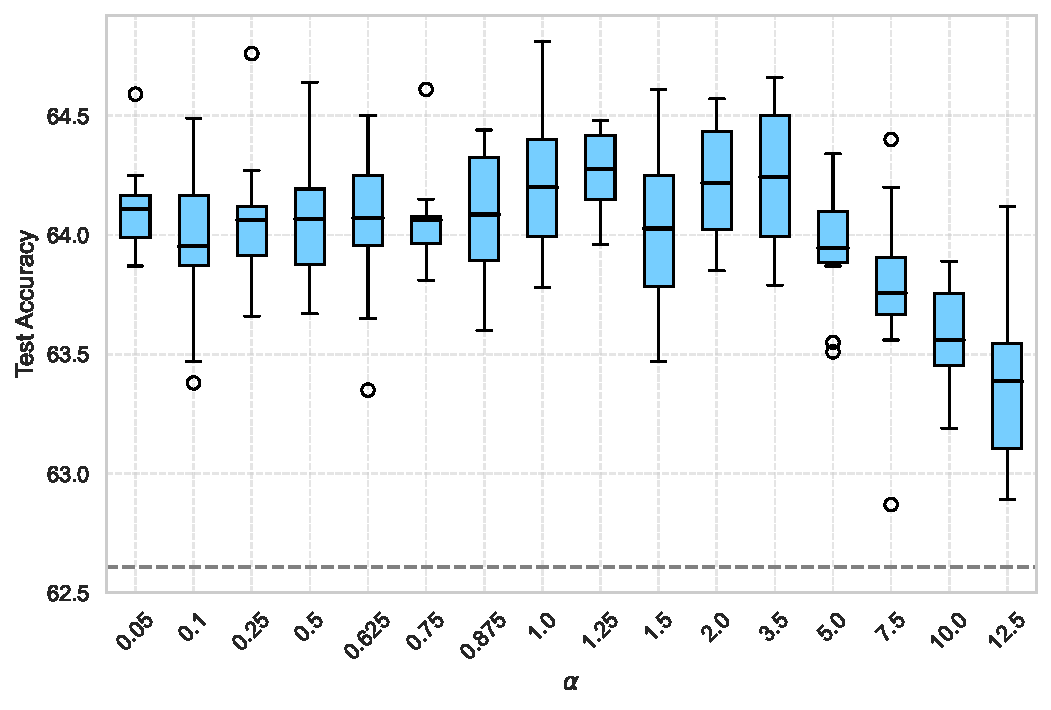
\includegraphics[width=0.7\textwidth]{../img/exp1_box_220.pdf}
	\caption{Boxplots of the performance of fully-trained models from Experiment 1, with average values indicated by black lines and the performance of the vanilla model represented by a dashed gray line.}
	\label{fig:exp1_box_219}
\end{figure}

Concentrating on the averages (and thus neglecting standard deviation), the models with values $\alpha$ between 1 and 3.5 perform the best. For $\alpha \geq 5$ the performance deteriorates, while still outperforming the vanilla model.

The most promising models are those with $\alpha = 1.25,\; 2,\; 3.5$. All of them outperform the standard knowledge distillation model, with $\alpha = 1.25$ achieving the best average accuracy of 64.277\%, which is 0.077\% higher than the accuracy for $\alpha = 1$. This further reduces the performance gap between the vanilla and teacher models by an additional 1.4\%, bringing the total reduction to 30.5\%.

These results, however, are not sufficient to conclude that choosing $\alpha = 1.25$ yields a statistically significant improvement over $\alpha = 1$. Nevertheless, we cannot rule out the possibility that this is indeed the case. More extensive testing is needed to draw definitive conclusions regarding this possibility.

In contrast, more promising results from a different perspective can be found in Figure~\ref{fig:exp1_box_10}, which depicts the performance of the models after only 10 epochs out of 220. It can be observed that only the student models corresponding to $\alpha$ values of 3.5, 5, or 7.5 significantly outperform the vanilla model. While lower values of $\alpha$ lead to deteriorating performance, both $\alpha = 1$ and $\alpha = 1.25$ trail behind the best-performing model with $\alpha = 5$.

\begin{figure}[h!]
	\centering
	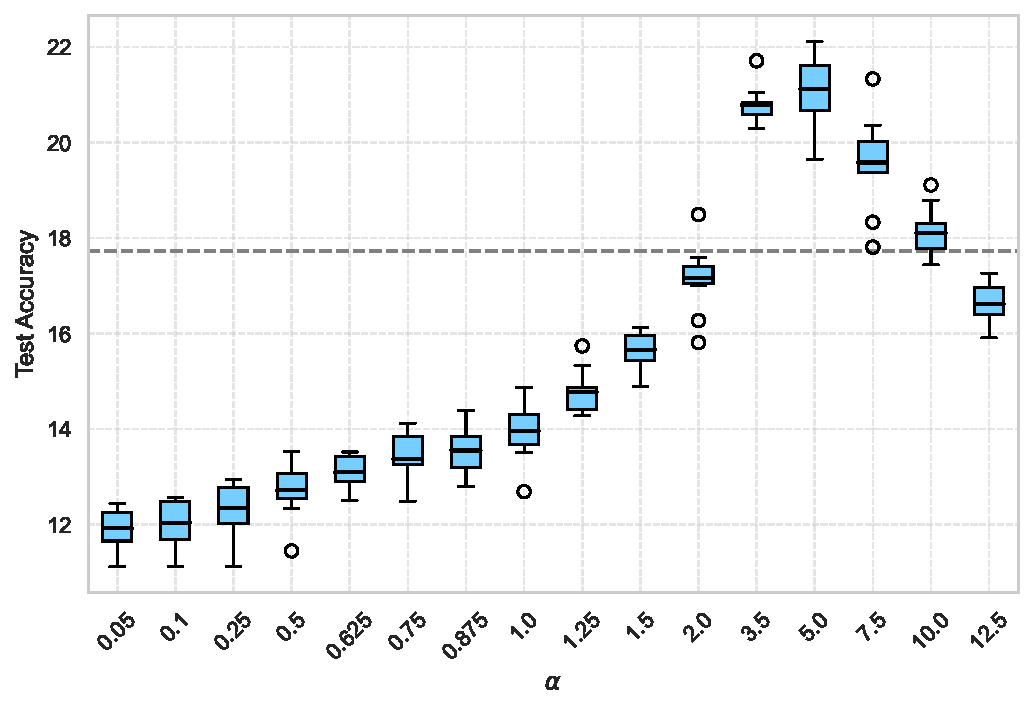
\includegraphics[width=0.7\textwidth]{../img/exp1_box_10.pdf}
	\caption{Boxplots of the performance of models from Experiment 1 after 10 epochs, with average values indicated by black lines and the performance of the vanilla model represented by a dashed gray line.}
	\label{fig:exp1_box_10}
\end{figure}

These results are not limited to the tenth epoch, as shown in Figure~\ref{fig:exp1_line_and_diff_plot}, which compares the aforementioned models, similar trends are observed across many early epochs of the training. This suggests that during training, higher values of $\alpha$ enable the student model to learn faster in the first few epochs.

The figure shows that the student model with $\alpha = 5$ outperforms all others in the early stages of training, with its advantage over the standard knowledge distillation model peaking around epochs 10 to 20 at approximately 5\% higher accuracy. The advantage shirks until epoch 70, where there is no longer any noticeable difference in performance. A similar pattern is observed for $\alpha = 1.25$, where the accuracy difference is smaller (around 1\%) but remains stable between epochs 10 and 50.

\begin{figure}[h!]
	\centering
	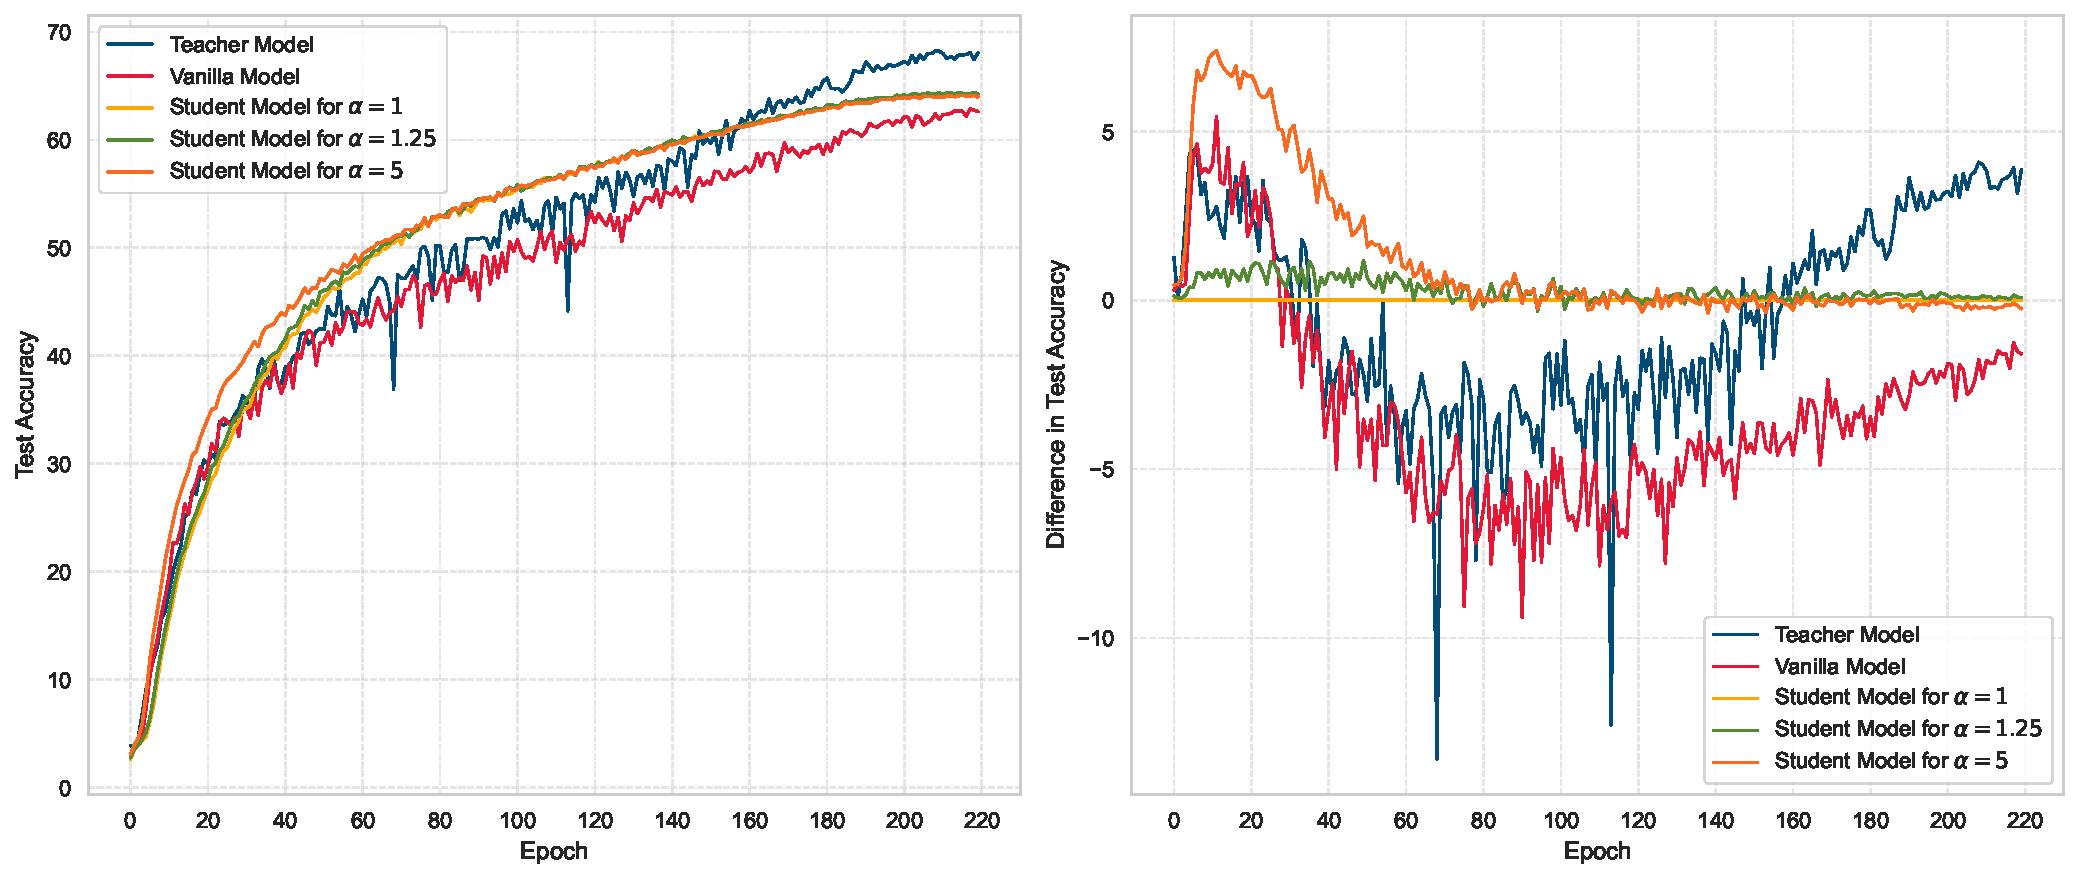
\includegraphics[width=1\textwidth]{../img/exp1_line_and_diff_plot.pdf}
	\caption{Comparison of the models. Left: Validation accuracy over 220 epochs for the teacher, vanilla, and selected student models. Right: Difference in accuracy compared to the student model with $\alpha=1$ over 220 epochs (Student models show averages over 10 iterations).}
	\label{fig:exp1_line_and_diff_plot}
\end{figure}

The performance difference between both the teacher and the vanilla models compared to the standard knowledge distillation model evolves over time. In the early stages, the vanilla-trained models slightly outperform the student model for $\alpha=1$, but around epoch 20, their performance begins to decline, and by epoch 90, they fall behind all student models by approximately 4\% in accuracy. After that point, both the teacher and the vanilla model continue to improve, albeit at different rates. While the teacher ultimately outperforms the student models, the vanilla model consistently remains behind all of them.

\section{Experiment 2}

This experiment extends the previous experiment by introducing two alternative formulations of the Rényi loss function from Equation~(\ref{Rényi loss}) and conducting tests similar to those in Experiment 1.

This has been motivated by the result of the preliminary testing. There we monitored various internal metrics of the student models, such as gradient behavior, to ensure that training with the Rényi loss function is numerically stable and exhibited well-conditioned optimization behavior. One of the monitored metrics is defined as

\begin{equation*}
	\kappa = \max_{(x,y) \in \mathcal{B},\, j} \left| \frac{v_j\, z_j}{T^2} \right|,
\end{equation*}
where $\mathcal{B}$ denotes the final batch of a given epoch, $v_j$ and $z_j$ the logits produced by the teacher and student models respectively, and $T$, the temperature hyperparameter, is fixed at 4.

This metric is connected to the assumption stated in Equation~\ref{assumption negligible}, particularly regarding the negligibility of the term $\frac{v_j z_j}{T^2}$. The assumption was used in deriving the result that the gradient of the Rényi loss function decreases proportionally to $\frac{\alpha}{T^2}$. This insight motivated the formulation of the Rényi loss function as shown in Equation~(\ref{Rényi loss}), which explicitly includes the scaling term $\frac{T^2}{\alpha}$.

Figure~\ref{fig:xy_T2} depicts the evolution of $\kappa$ during training, showing a steady increase over time, ultimately reaching approximately 5.5. Thus, it is evident that the assumption of negligibility of $\frac{v_j z_j}{T^2}$ does not generally hold.

\begin{figure}[h!]
	\centering
	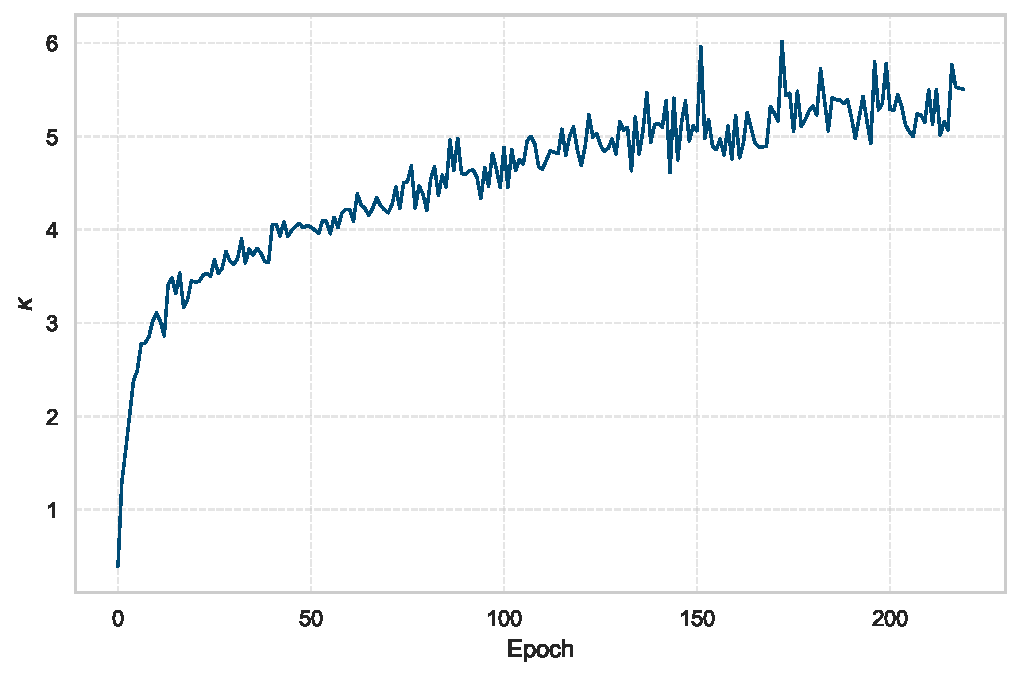
\includegraphics[width=0.7\textwidth]{../img/xy_T2.pdf}
	\caption{Average value of $\kappa$ during testing across all models, computed by averaging over various values of $\alpha$, with $T=4$, as observed in the preliminary testing.}
	\label{fig:xy_T2}
\end{figure}

This behavior arises from the temperature not being sufficiently high. However, as noted in the case of standard knowledge distillation by \cite{HintonVinyalsDean2015}, this may not be a critical issue. In any case, this prompted us to examine how the gradient of the Rényi loss function with respect to the logits of the student model behaves as a function of the hyperparameter $\alpha$.

In the previous experiment, we observed that the performance of student models corresponding to different values of $\alpha$ diverges most significantly at the beginning of the training. Thus, we focus on the initial phase of the training, using an untrained ResNet18 model as the student and a fully-trained ResNet101 model on CIFAR-100 as the teacher. To calculate the gradient we use Equation~(\ref{Rényi gradient}).

We calculate the gradients for 1,000 images from the training set, resulting in 100,000 different values, as each image produces 100 values corresponding to the 100 classes. Both the teacher and the student output a prediction by selecting the class with the highest logit among the 100 possible classes. We use this prediction to label the gradients. We assign a label of 11 to a value if the corresponding class is predicted by both models. A label of 10 is assigned if only the teacher predicts the class, 1 if only the student model does, and 0 if neither.

We expect the vast majority of the values to be labeled as 0, since each model predicts only one class out of 100. Since the untrained student model is essentially a random number generator, it always predicts a random class. As a result, only a small number of values will be labeled as 11, that is predicted by both models simultaneously.

The motivation for introducing these labels is that, for both fully trained models, classes 1, 10, and 11 correspond to high logit values produced by the student, the teacher, and both models, respectively. Without separating them from class 0, these values would appear as outliers. This is undesirable, as the behavior of these values provides valuable insight into the training process.

Figure~\ref{fig:gradients_boxplot_adjusted} shows the gradients in form of boxplots for different values of $\alpha$, grouped according to their assigned labels. We observe, that the behavior of classes 0 and 1 are similar, the same is true for classes 10 and 11. This again results from the fact that the student model is untrained, so the largest logit is expected to have a similar magnitude to the other logits. This would not be true for trained student model.

\begin{figure}[h!]
	\centering
	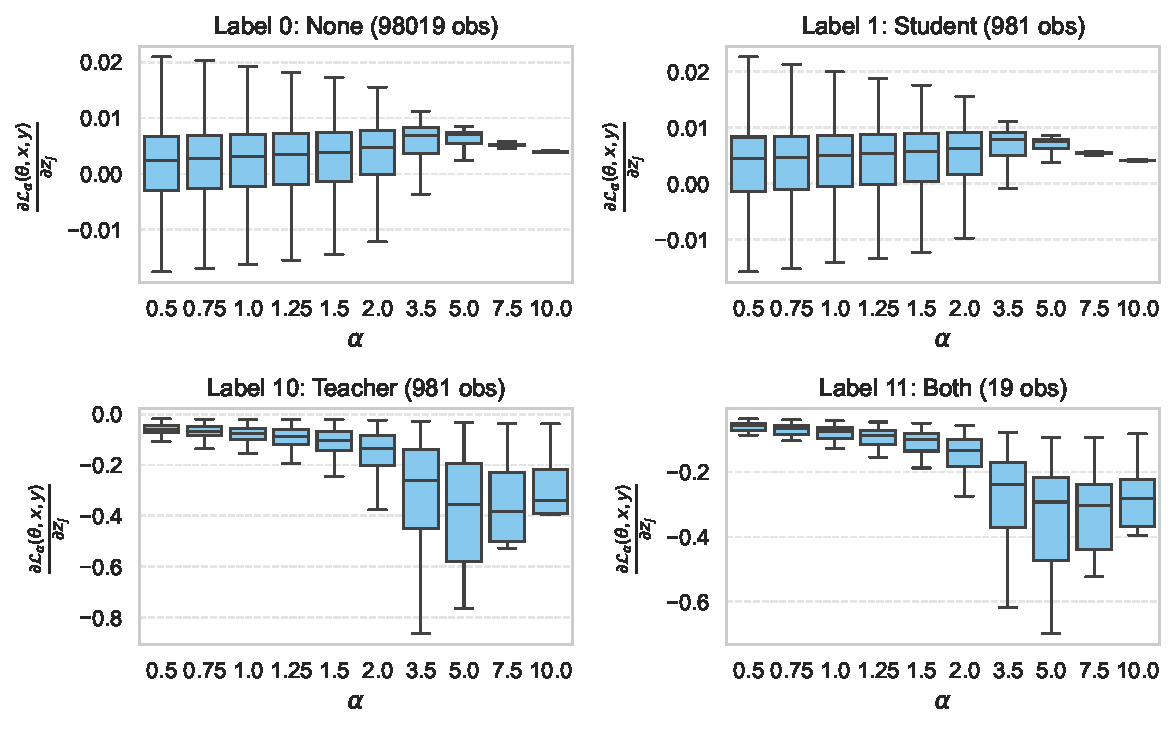
\includegraphics[width=0.7\textwidth]{../img/gradients_boxplot_adjusted.pdf}
	\caption{Boxplots of the gradient values of the Rényi loss with respect to the student model logits, across various values of $\alpha$, grouped by label, for $T=4$.}
	\label{fig:gradients_boxplot_adjusted}
\end{figure}

The differences in gradients for varying values of $\alpha$ for labels 1, 10 and 11 are desirable, as they represent one of the key factors that cause the training process to differ across values of $\alpha$. What may be considered undesirable, however, is the variation in the medians for label 0, as it suggests an inconsistent learning rate across different settings, especially for larger values of $\alpha$. Additionally, we observe that the variance decreases, which might be one of the factors contributing to the lower performance observed for larger values of $\alpha$ in Experiment 1.

There are two approaches we might consider. Firstly, since the conditions required to simplify the derivative of the Rényi divergence are quite restrictive, we might choose not to use the scaling term $\frac{T^2}{\alpha}$. Instead, we consider a solution which has been already used by \cite{HintonVinyalsDean2015} for the case of the standard knowledge distillation and might be a viable in our case. There, we simply replace the KL divergence with the Rényi divergence in Equation~(\ref{KL loss}), resulting in the following unscaled Rényi loss function

\begin{equation}
	\mathcal{L}_{\alpha,\text{unscaled}}(\theta,x,y) = T^2 D_\alpha(P^T \| Q^T).
	\label{modified_RL_noadj}
\end{equation}

Alternatively, we may aim to find a scaling function $\phi(\alpha,T)$ that keeps the median of the gradients for label 0 constant across varying values of $\alpha$, thereby normalizing them, resulting in the normalized Rényi loss function

\begin{equation}
	\mathcal{L}_{\alpha,\text{norm}}(\theta,x,y) = \phi(\alpha,T) D_\alpha(P^T \| Q^T).
	\label{modified_RL_sigmoid}
\end{equation} 

\paragraph{Unscaled loss} In Figure~\ref{fig:gradients_boxplot_noadj} and, we present a graphs analogous to Figure~\ref{fig:gradients_boxplot_adjusted}, calculated using the unscaled loss function given in Equation~(\ref{modified_RL_noadj}). There, we observe that the median of the gradients for label 0 varies even more across different values of $\alpha$, compared to the previous approach. This implies that changing $\alpha$ indirectly affects the effective learning rate. One of the implications is the possibility of better performance of the student model during the initial epochs. Also note that the variance differs, peaking at $\alpha = 2$, while becoming particularly small for larger values of $\alpha$.

\begin{figure}[h!]
	\centering
	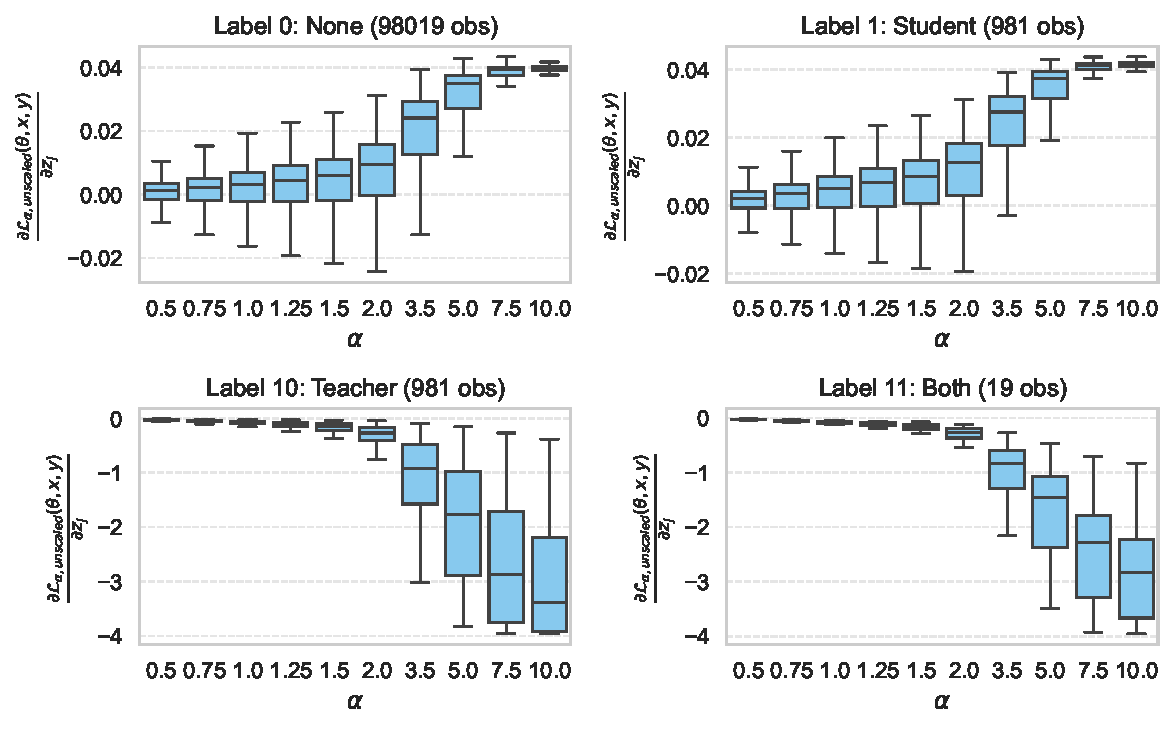
\includegraphics[width=0.7\textwidth]{../img/gradients_boxplot_noadj.pdf}
	\caption{Boxplots of the gradient values of the unscaled Rényi loss from Equation~(\ref{modified_RL_noadj}) with respect to the student model logits, across various values of $\alpha$, grouped by label, for $T=4$.}
	\label{fig:gradients_boxplot_noadj}
\end{figure}

For the second approach, we need to estimate the function $\phi(\alpha,T)$. We require that $\phi(1,T)=T^2$, as this ensures the training process is equivalent to standard knowledge distillation, i.e., when $\alpha=1$. In our case, we focus exclusively on $T=4$, as this is the temperature used in all experiments.

We first estimate the behavior of the gradients when setting $\phi(\alpha,T)=T^2$ for all values of $\alpha$, which reduces the normalized loss function from Equation~(\ref{modified_RL_sigmoid}) to the form given in Equation~(\ref{modified_RL_noadj}). Thus, we can use the results from Figure~\ref{fig:gradients_boxplot_noadj} as a reference while computing additional values for other settings of $\alpha$. These results can be seen in Figure~\ref{fig:sigmoid_approx}. We immediately recognize the shape of the curve as resembling a sigmoid-like function. Therefore, we fit a sigmoid function to the data, denoted as $\sigma(\alpha)$ which, upon fitting, is given by the following expression

\begin{equation*}
	\hat{\sigma}(\alpha) = \frac{0.0416}{1 + e^{-(0.9968\, \alpha - 2.9970)}} - 0.0018.
\end{equation*}
The relationship between the function $\sigma(\alpha)$ and $\phi(\alpha,4)$ is as follows

\begin{equation*}
	\phi(\alpha,4) = \frac{\sigma(1)}{\sigma(\alpha)} 4^2,
\end{equation*}
since $\sigma(\alpha)$ approximates the median of the gradients labeled as 0, dividing the loss function by $\sigma(\alpha)$ results in a constant median of these gradients. Additionally, $\phi(1,4)=4^2$, as required.

\begin{figure}[h!]
	\centering
	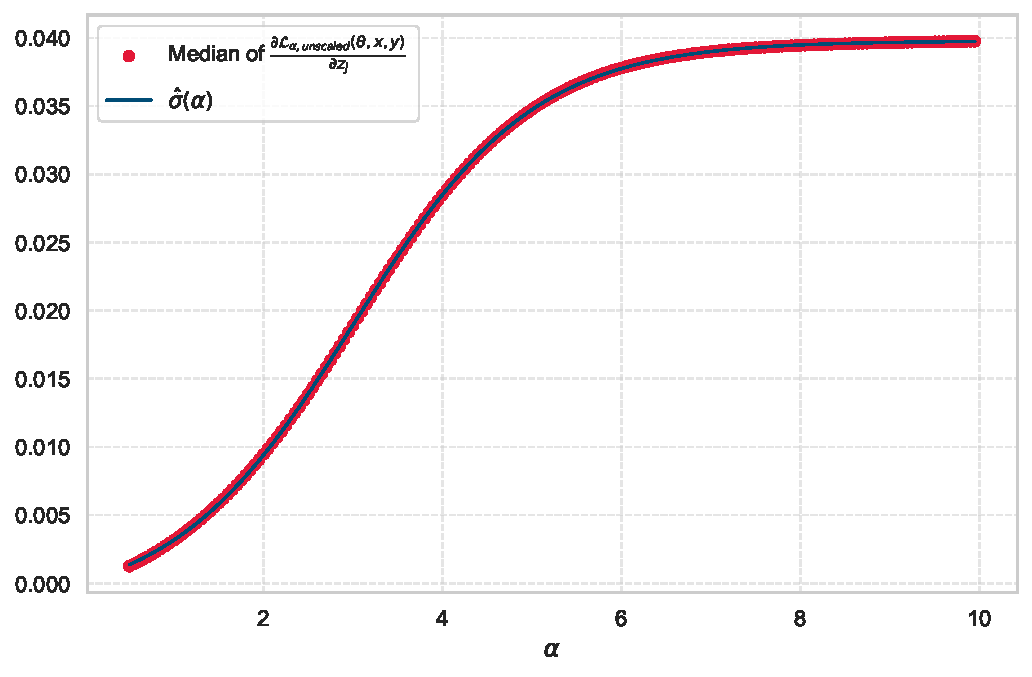
\includegraphics[width=0.7\textwidth]{../img/sigmoid_approx.pdf}
	\caption{Medians of gradient values for label 0, computed using the unscaled Rényi loss from Equation~(\ref{modified_RL_noadj}) with respect to the student model logits, across various values of $\alpha$, along with the function $\hat{\sigma}(\alpha)$ estimated from this data}
	\label{fig:sigmoid_approx}
\end{figure} 

Using this approach with the fitted $\hat{\phi}(\alpha,4)$, we compute the gradients analogously to the previous figures, resulting in Figure~\ref{fig:gradients_boxplot_sigmoid}. As observed, the medians of the gradients for label 0 remain constant, as intended. The variance diminishes with increasing $\alpha$, similarly to the case of the original Rényi-based knowledge distillation.

\begin{figure}[h!]
	\centering
	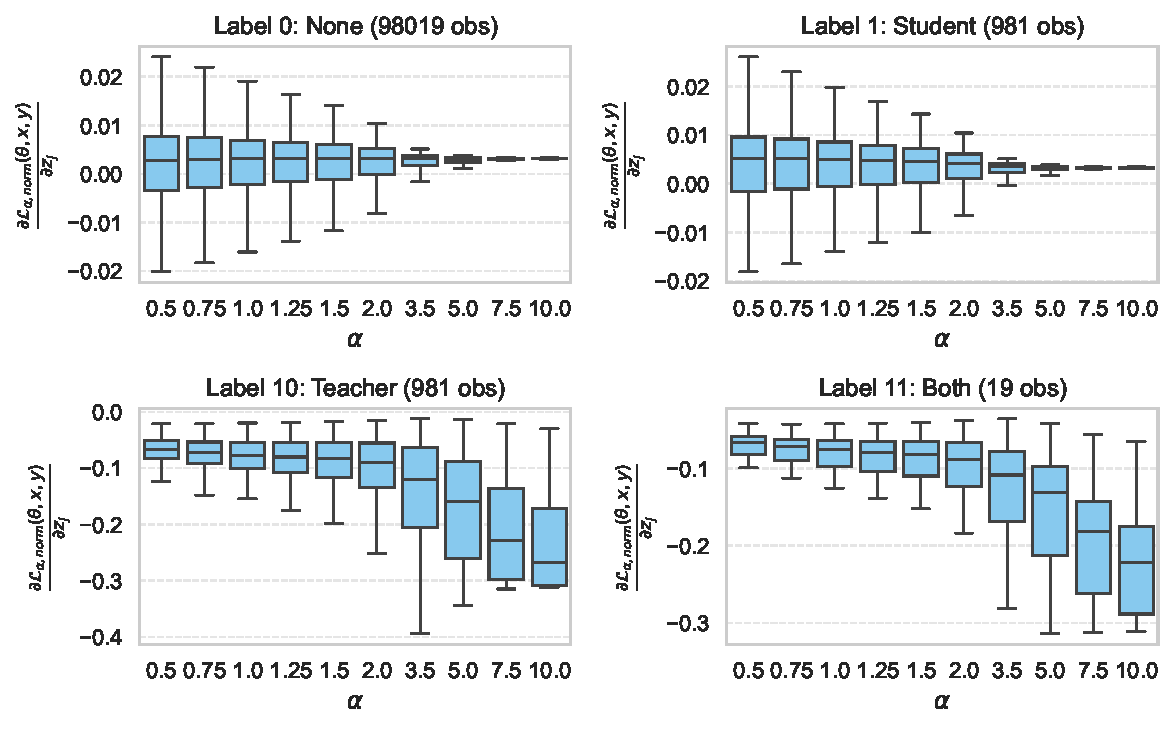
\includegraphics[width=0.7\textwidth]{../img/gradients_boxplot_sigmoid.pdf}
	\caption{Boxplots of the gradient values of the normalized Rényi loss from Equation~(\ref{modified_RL_sigmoid}) with respect to the student model logits, across various values of $\alpha$, grouped by label, for $T=4$.}
	\label{fig:gradients_boxplot_sigmoid}
\end{figure}

Following the introduction of the two approaches and a brief analysis of their gradients, we aim to directly compare them to the results of Experiment 1 using the CIFAR-100 dataset. We now train student model for each choice of $\alpha$ from the Table~\ref{tab:exp2_res} with modified Rényi knowledge distillation with 10 different seeds. As before, we report the average test accuracy, with the accuracy improvement over the vanilla model shown as a superscript.

\begin{table}[h]
	\centering
	\begin{tabular}{lccc}
		\toprule
		$\boldsymbol{\alpha}$ & $\bf{Original}$ & $\bf{Unscaled}$ & $\bf{Normalized}$ \\ \midrule
		0.5 & $64.067^{1.457}$ & $63.855^{1.245}$ & $64.367^{1.757}$ \\
		0.625 & $64.072^{1.462}$ & $64.099^{1.489}$ & $64.216^{1.606}$ \\
		0.75 & $64.062^{1.452}$ & $63.961^{1.351}$ & $64.295^{1.685}$ \\
		0.875 & $64.086^{1.476}$ & $64.206^{1.596}$ & $64.297^{1.687}$ \\
		1.0 & $64.200^{1.590}$ & $64.281^{1.671}$ & $64.311^{1.701}$ \\
		1.25 & $\bf{64.277^{1.667}}$ & $\bf{64.499^{1.889}}$ & $64.196^{1.586}$ \\
		1.5 & $64.027^{1.417}$ & $64.370^{1.760}$ & $\bf{64.373^{1.763}}$ \\
		2.0 & $64.218^{1.608}$ & $64.480^{1.870}$ & $64.343^{1.733}$ \\
		3.5 & $64.242^{1.632}$ & $64.130^{1.520}$ & $64.042^{1.432}$ \\
		5.0 & $63.946^{1.336}$ & $64.246^{1.636}$ & $64.034^{1.424}$ \\
		7.5 & $63.757^{1.147}$ & $63.802^{1.192}$ & $63.868^{1.258}$ \\
		\bottomrule
	\end{tabular}
	\caption{Results of Experiment 2 showing the average test accuracy for various values of $\alpha$, with the improvement over the vanilla model in superscript. The best result for each loss function is highlighted in bold.}
	\label{tab:exp2_res}
\end{table}

First, we note that for $\alpha=1$, all approaches are equivalent. That being said, the results for different loss functions shown in the table differ noticeably, suggesting that the average accuracy of the model over ten seeds can fluctuate by more than 0.1\%. Therefore, any difference within 0.1\% should not be considered statistically significant.

The best performance was achieved with $\alpha=1.25$ and the unscaled loss function, achieving an average accuracy of 64.449\%, which is 1.889\% higher than the vanilla model and 0.222\% higher than the best model from Experiment 1. Furthermore, it reduces the gap between the vanilla model and the teacher by 34.7\%, which is 4.2\% more than the reduction achieved by the best model using the original loss function. The best model using the normalized loss adjustment, achieved with $\alpha=1.5$, also outperforms the best model from Experiment 1, though only by 0.096\%.

\begin{figure}[h!]
	\centering
	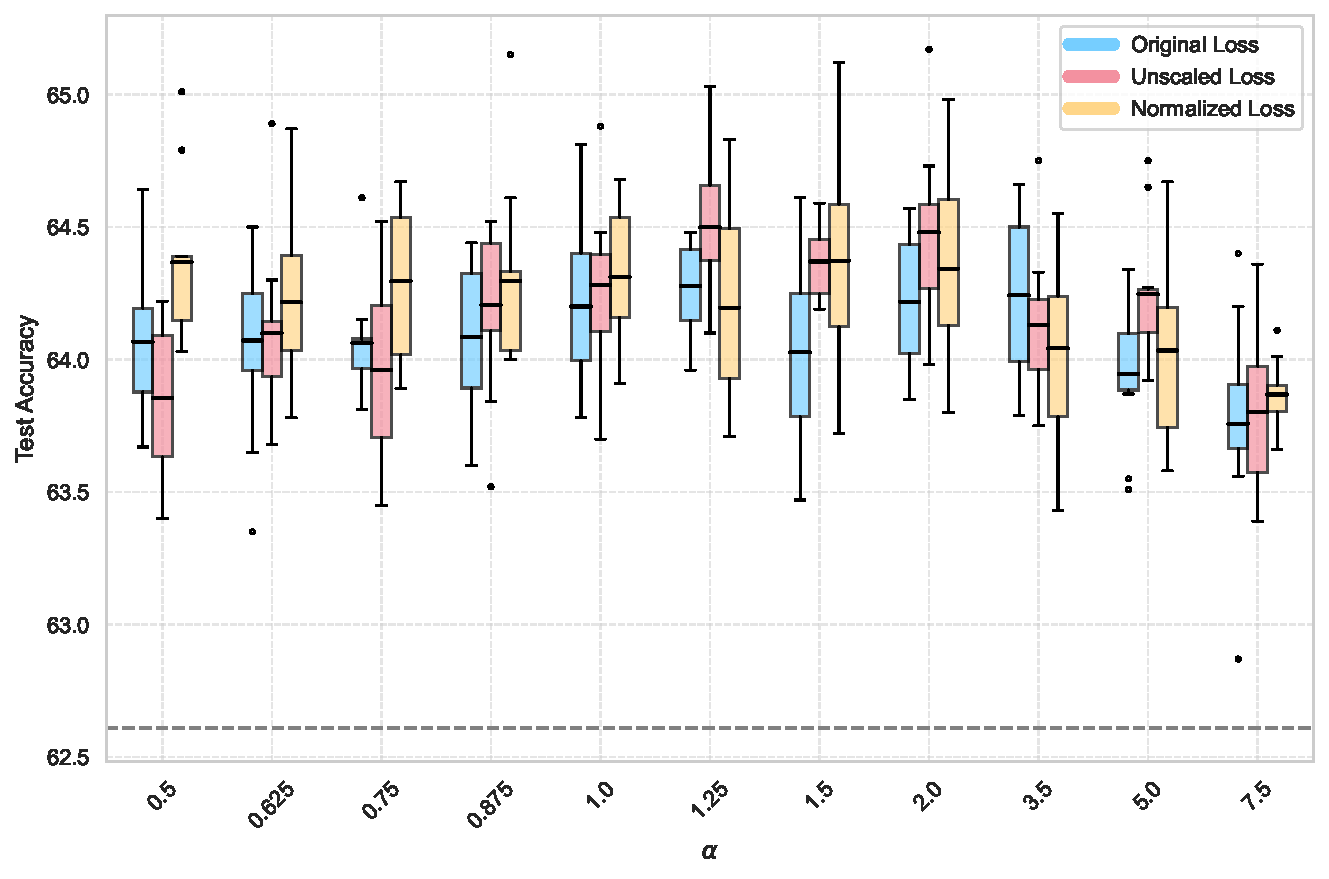
\includegraphics[width=0.7\textwidth]{../img/exp2_box_grouped_220.pdf}
	\caption{Boxplots of the performance of fully-trained models from Experiment 2, with mean values indicated by black lines and the performance of the vanilla model represented by a dashed gray line.}
	\label{fig:exp2_box_grouped_220}
\end{figure}

Figure~\ref{fig:exp2_box_grouped_220} shows the unaggregated results in the form of boxplots. From the figure, it is clear that the models utilizing the unscaled Rényi loss function achieve the best performance compared to the other approaches for $\alpha$ values between 1.25 and 2. Conversely, for $\alpha$ values below 0.75, these models perform the worst on average. For $\alpha$ greater than 3.5 the accuracy decreases across all models.

Interestingly, the performance of models using the normalized loss function remains relatively constant for all $\alpha$ values up to 3.5. Additionally, for all $\alpha$ values except 1.25, the average accuracy exceeds that of the student models trained with the original loss function.

Looking at Figure~\ref{fig:exp2_box_grouped_10}, which shows the performance of the models after only 10 out of 220 training epochs, we observe that the student models of the unscaled loss exhibit the most extreme behavior, achieving nearly 30\% accuracy for $\alpha \geq 3.5$, but failing to reach even 10\% for $\alpha=0.5$. This is most probably due to the difference in the gradients we have observed in Figure~\ref{fig:gradients_boxplot_noadj}. This, in turn, affects the effective learning rate, which then might result in lower performance of the models with low hyperparameter $\alpha$.

\begin{figure}[h!]
	\centering
	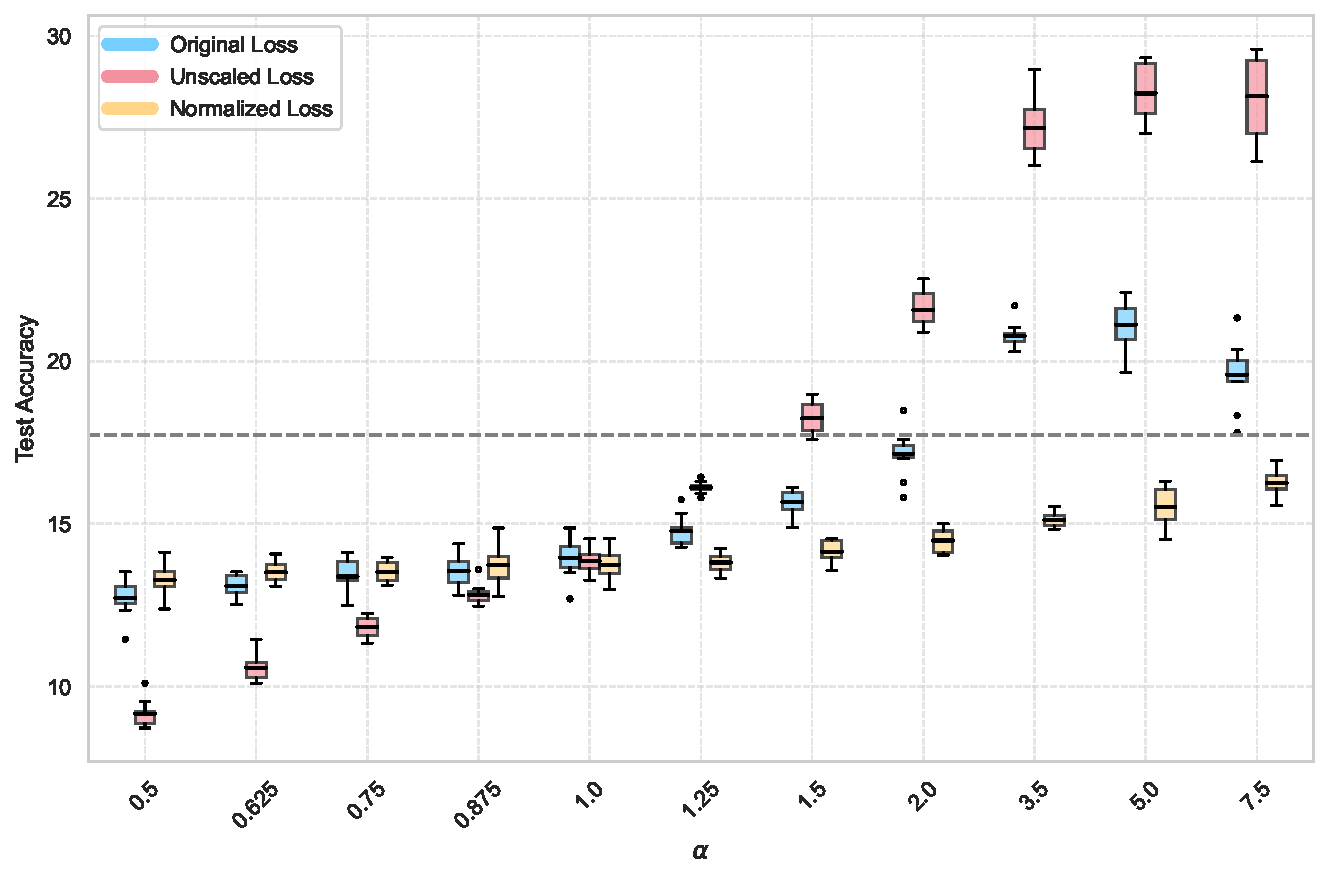
\includegraphics[width=0.7\textwidth]{../img/exp2_box_grouped_10.pdf}
	\caption{Boxplots of the performance of models from Experiment 2 after 10 epochs, with mean values indicated by black lines and the performance of the vanilla model represented by a dashed gray line.}
	\label{fig:exp2_box_grouped_10}
\end{figure}

Turning our attention to the student models trained with the normalized Rényi loss function, we observe that their performance remains much more consistent across different values of $\alpha$. However, there is still a difference, where the accuracy for $\alpha>3.5$ is around 15\% after 10 epochs, but only about 13\% for $\alpha=0.5$. This implies that higher $\alpha$ values improve performance early in training, not only by increasing the effective learning rate but also through other factors.

\begin{figure}[h!]
	\centering
	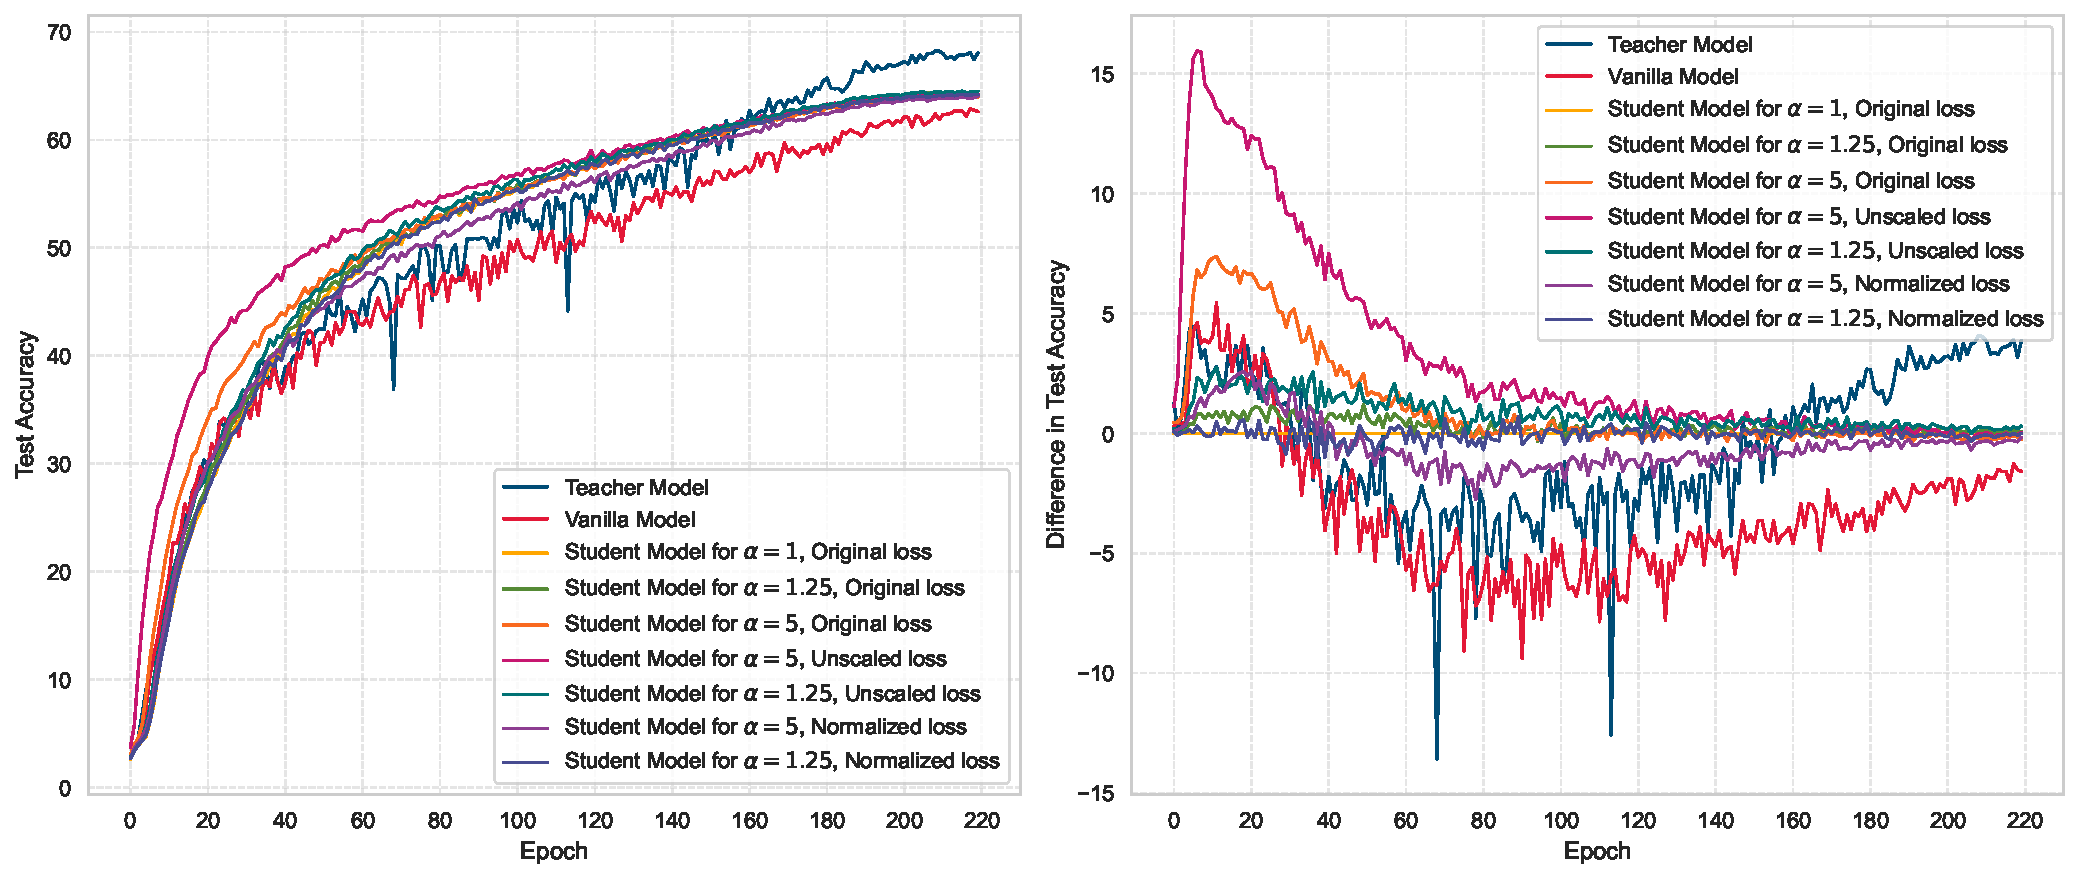
\includegraphics[width=1\textwidth]{../img/exp2_line_and_diff_plot.pdf}
	\caption{Comparison of the models with modified loss function. Left: Validation accuracy over 220 epochs for the teacher, vanilla, and selected student models. Right: Difference in accuracy compared to the student model with $\alpha=1$ over 220 epochs (Student models show averages over 10 iterations).}
	\label{fig:exp2_line_and_diff_plot}
\end{figure}

Lastly, Figure~\ref{fig:exp2_line_and_diff_plot} shows the performance of the various student models over the entire training process, rather than at a single epoch. Additionally, the plot on the right shows the difference in accuracy between these models and the student model trained with standard knowledge distillation.

We observe that models using the unscaled Rényi loss function with $\alpha = 5$ not only achieve the best performance at epoch 10, but also maintain this lead for a substantial portion of the training, remaining the top performers for approximately 120 epochs. This difference, when compared to the models trained with standard knowledge distillation, peaks around epoch 10, reaching approximately 15\%. When examining the models with the same loss function but using $\alpha = 1.25$, we observe that they outperform standard knowledge distillation during the initial epochs, though the difference is smaller, only about 2\%. This advantage gradually diminishes but remains noticeable until around epoch 120.

When comparing models trained with the unscaled loss to those using the original loss, we observe that the advantage over standard knowledge distillation peaks around the same epoch in both cases, but the gap is larger for the unscaled loss. Moreover, while the original loss shows a noticeable advantage for about 70 epochs, the unscaled version maintains this advantage for approximately 120 epochs.

On the other hand, the training process using the normalized loss behaves quite differently. For $\alpha = 1.25$, its behavior closely mirrors that of standard knowledge distillation, showing essentially no distinction. While for $\alpha = 5$, the normalized loss results in higher performance, with about 2\% better accuracy after 10 to 20 epochs. By epoch 40, the performances are nearly the same. However, after that point, the standard model begins to perform better, with the difference in accuracy reaching a peak of approximately 1\% around epoch 80. Although the gap becomes smaller again toward the end of training, the normalized model ultimately performs about 0.2\% worse.

\section{Discussion}

The first experiment confirmed the known benefits of knowledge distillation, which consistently outperformed the vanilla student model. More notably, models with values of $\alpha$ within the range of 1 to 3.5 produced better results than the standard knowledge distillation. However, these improvements were not statistically significant under conventional thresholds, and thus require further investigation through larger-scale experiments.

Interestingly, the early stages of training revealed a different dynamic. Higher values of $\alpha$ (e.g., 3.5 or 5) led to a higher test accuracy in the early stages of training. This suggests that larger values of $\alpha$ might be particularly useful in settings where early convergence or rapid experimentation is desirable. This advantage diminishes as training progresses and does not translate to better final performance.

In the second experiment, we proposed two alternatives to the Rényi loss function used in knowledge distillation, by modifying the scaling term, as we feared the higher performance in early stages was due to higher effective learning rate. Both strategies aimed to reduce this indirect influence of $\alpha$, either by applying a constant scaling across different values of $\alpha$ (unscaled Rényi loss function), or by adjusting it based on the behavior of the median of gradients (normalized Rényi loss function).

The results showed that the unscaled loss function slightly outperformed both the original and normalized versions, with the best performance achieved at $\alpha = 1.25$. The normalized version also surpassed the original and had consistent performance across all values of $\alpha$ between 0.5 and 3.5.

In the early stages, models with high $\alpha$ using the unscaled loss function performed best, which we attribute to their higher effective learning rate, as we observed that this approach does not normalize the means of the gradients. The performance advantage of models with high $\alpha$ using the unscaled normalized function was not as high, but it was still present, suggesting that higher values of $\alpha$ improve performance in the early phases of training, not only by increasing the effective learning rate.

Despite the promising results, it is important to stress that all testing was conducted on a small scale using the CIFAR-100 dataset. For a more conclusive evaluation of our proposed methods, we recommend testing on a much larger scale, such as with the ImageNet dataset (see \cite{Deng2009}).

Further research might also include tuning other introduced hyperparameters, such as $\beta$ and temperature $T$, in addition to standard hyperparameters like learning rate and weight decay. There may also be potential in creating a dynamic schedule for the hyperparameter $\alpha$, changing it during the training process for faster convergence and better performance. Calculating the function $\phi(\alpha,T)$ from Equation~\ref{modified_RL_sigmoid} for values of $T \neq 4$, or deriving an analytical solution, as well as focusing on the effect variance of gradients, which differs for various values of $\alpha$ and different Rényi loss functions, could be interesting directions for further work.







